\documentclass[11pt]{beamer}
\beamertemplatenavigationsymbolsempty
\usetheme{Penn} 

\logo{}


\usepackage{epsfig, amsfonts, amsbsy, amsmath}
\usepackage{color}
\usepackage{amsmath}
\usepackage{amssymb}
\usepackage{scrextend}
\usepackage{float}
\usepackage{color}
\usepackage{graphicx} 
\usepackage{caption}
\usepackage{subcaption}
\usepackage{url}
\usepackage{natbib}


% Copyright 2007 by Till Tantau
%
% This file may be distributed and/or modified
%
% 1. under the LaTeX Project Public License and/or
% 2. under the GNU Public License.
%
% See the file doc/licenses/LICENSE for more details.

\ProvidesPackageRCS $Header: /cvsroot/latex-beamer/latex-beamer/themes/color/beamercolorthemepenn.sty,v 1.4 2007/01/28 20:48:24 tantau Exp $

\definecolor{pennred}{cmyk}{0.75, 0.4, 1, 0.4}
\definecolor{pennblue}{cmyk}{1,0.7,0,0.30}



\mode<presentation>

\setbeamercolor*{palette primary}{use=structure,fg=white,bg= pennblue}
\setbeamercolor*{palette secondary}{use=structure,fg=white,bg= pennblue}
\setbeamercolor*{palette tertiary}{use=structure,fg=white,bg= pennblue}
\setbeamercolor*{palette quaternary}{fg=white,bg= pennblue}

\setbeamercolor*{sidebar}{use=structure,bg= pennblue}
  
\setbeamercolor*{palette sidebar primary}{use=structure,fg=structure.fg!10}
\setbeamercolor*{palette sidebar secondary}{fg=white}
\setbeamercolor*{palette sidebar tertiary}{use=structure,fg=structure.fg!50}
\setbeamercolor*{palette sidebar quaternary}{fg=white}

\setbeamercolor*{titlelike}{parent=palette primary}

\setbeamercolor*{separation line}{}
\setbeamercolor*{fine separation line}{}

\setbeamercolor{itemize item}{fg=pennblue}
\setbeamercolor{itemize subitem}{fg=pennblue}
\setbeamercolor{itemize subsubitem}{fg=pennblue}
\setbeamercolor{enumerate item}{fg=pennblue}
\setbeamercolor{enumerate subitem}{fg=pennblue}
\setbeamercolor{enumerate subsubitem}{fg=pennblue}
\setbeamercolor{description item}{fg=pennblue}


\mode
<all>

 \setbeamercovered{invisible}
 

\begin{document}

\author[]{\begin{tabular}{c} 
\\ \textbf{Team:} \\
{\small Individual 1}\\
{\small Individual 2}\\
{\small Individual 3}\\
{\small ... (order names alphabetically)}
\end{tabular}}

\date{Spring 2019}

\title{Project Topic}


\frame{
\begin{center}
{\small Fairness, Explainability, and Accountability for ML}
\end{center}
\titlepage}

\begin{frame}{Title}
\begin{itemize}
\item Sample text
\end{itemize}
\end{frame}

\begin{frame}{Sample Image}
\begin{itemize}
\item All figures must be places in the ``Figures" folder.
\end{itemize}
\begin{figure}[t!]
    \centering
        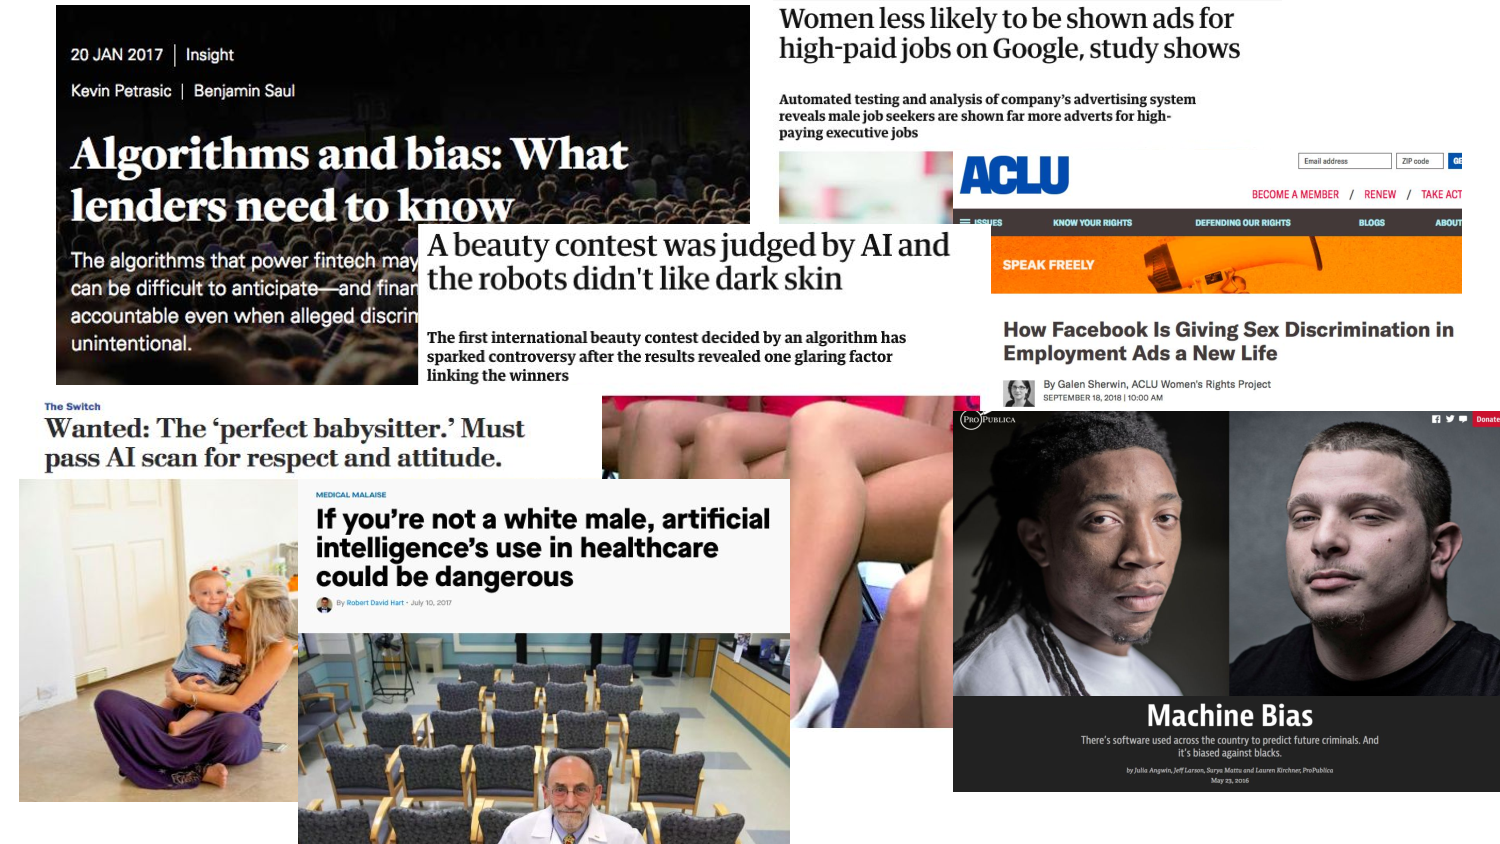
\includegraphics[width=0.5\textwidth]{Figures/media_negative.pdf}
\end{figure}
\end{frame}


\begin{frame}{References}
\begin{itemize}
\item All relevant resources (articles, softwares, etc.) must be listed at the end of the presentation.
\end{itemize}
\end{frame}

\end{document}
